\documentclass{zc-ust-hw}

\usepackage[label=corner]{karnaugh-map} 
\usepackage{caption} 
\usepackage{circuitikz}
\usepackage{enumitem}
\usepackage{floatrow}
\usepackage{lipsum}
\usepackage{listings}
\usepackage{newfloat}
\usepackage{subcaption}
\usepackage{xcolor}

\newenvironment{solution}
  {\renewcommand\qedsymbol{$\blacksquare$}\begin{proof}[Solution]}
  {\end{proof}}

\DeclareFloatingEnvironment[fileext=lop]{K-Map}

\lstdefinestyle{SystemVerilogStyle}{
    language=Verilog,
    basicstyle=\small\ttfamily,
    keywordstyle=\color{blue}\bfseries,
    commentstyle=\color{green!60!black},
    morecomment=[l]{//},
    morecomment=[s]{/*}{*/},
    stringstyle=\color{orange},
    breaklines=true,
    showstringspaces=false,
    numbers=left,
    numberstyle=\tiny,
    numbersep=5pt,
    backgroundcolor=\color{gray!10},
    frame=single,
    rulecolor=\color{black!40},
    captionpos=b,
    tabsize=4,
    morekeywords={module, endmodule, input, output, reg, always, begin, end, if, else, for, while, case, endcase}
}

\newcommand*{\name}{SalahDin Rezk}
\newcommand*{\id}{202201079}
\newcommand*{\course}{Digital Design and Computer Architecture (CIE 239)}
\newcommand*{\assignment}{Assignment 2}

\begin{document}

\maketitle

\begin{enumerate}

  \item 
    \begin{enumerate}[label=\alph*.]
      \item Write a Boolean equation in sum-of-products canonical form and
        product-of-sum canonical form for following truth table. 
        \begin{table}[htpb]
          \centering
          \begin{tabular}{cccc|c}
            $A$ & $B$ & $C$ & $D$ & $Y$ \\
            \hline
            0 & 0 & 0 & 0 & 1 \\
            0 & 0 & 0 & 1 & 1 \\
            0 & 0 & 1 & 0 & 1 \\
            0 & 0 & 1 & 1 & 1 \\
            0 & 1 & 0 & 0 & 0 \\
            0 & 1 & 0 & 1 & 0 \\
            0 & 1 & 1 & 0 & 0 \\
            0 & 1 & 1 & 1 & 0 \\
            1 & 0 & 0 & 0 & 1 \\
            1 & 0 & 0 & 1 & 0 \\
            1 & 0 & 1 & 0 & 1 \\
            1 & 0 & 1 & 1 & 0 \\
            1 & 1 & 0 & 0 & 0 \\
            1 & 1 & 0 & 1 & 0 \\
            1 & 1 & 1 & 0 & 1 \\
            1 & 1 & 1 & 1 & 0 \\
          \end{tabular}
          \caption{}
          \label{tab:1}
        \end{table}
        \begin{solution}
          \begin{align}
            Y &= A'B'C'D'+A'B'C'D+A'B'CD'+A'B'CD+AB'C'D'+AB'CD'+ABCD' \\
            &= \Sigma(0,1,2,3,8,10,14)
          .\end{align}
          \begin{align}
            Y &=
            \begin{array}{l}
              (A+B'+C+D)(A+B'+C+D')(A+B'+C+D')(A+B'+C'+D) \\
              (A+B'+C'+D')(A'+B+C+D')(A'+B+C'+D')(A'+B'+C+D) \\
              (A'+B'+C+D') (A'+B'+C'+D')
            \end{array}\\
              &= \Pi(4,5,6,7,9,11,12,13,15)
          .\end{align}
        \end{solution}
        \newpage
      \item Minimize each of the Boolean equations of the sum-of products (use
        Boolean algebra) and implement the simplified equation using basic
        logic gates (AND, OR and NOT gate). 
        \begin{solution}
          \begin{align}
            Y &= A'B'C'D'+A'B'C'D+A'B'CD'+A'B'CD+AB'C'D'+AB'CD'+ABCD' \\
              &= A'B'C'(D'+D)+A'B'CD'+A'B'CD+AB'D'(C'+C)+ABCD' \\
              &= A'B'C'+A'B'CD'+A'B'CD+AB'D'+ABCD' \\
              &= A'B'(C'+CD')+A'B'CD+AB'D'+ABCD' \\
              &= A'B'(C'+D')+A'B'CD+AB'D'+ABCD' \\
              &= A'B'(C'+D'+CD)+AB'D'+ABCD' \\
              &= A'B'(C'+CD+D')+AB'D'+ABCD' \\
              &= A'B'(C'+D+D')+AB'D'+ABCD' \\
              &= A'B'(C'+1)+AB'D'+ABCD' \\
              &= A'B'+AB'D'+ABCD' \\
              &= B'(A'+AD')+ABCD' \\
              &= B'(A'+D')+ABCD' \\
              &= A'B' + B'D' + ABCD' \\
              &= A'B' + D'(B' + ABC) \\
              &= A'B' + D'(B' + BAC) \\
              &= A'B' + D'(B' + AC) \\
              &= A'B' + B'D' + ACD'
          .\end{align}
          \begin{figure}[htpb]
            \begin{center}
              \begin{circuitikz}
                % Inputs
                \draw (0,0) node[above] {$A$} to[short] (0,-4.5);
                \draw (0.5,0) node[above] {$B$} to[short] (0.5,-2.5);
                \draw (1,0) node[above] {$C$} to[short] (1,-5);
                \draw (1.5,0) node[above] {$D$} to[short] (1.5,-5.5);
                % OR gate
                \draw (8,-3) node[or port, number inputs=3] (or1) {}
                (or1.out) node[right] {$Y$};
                % AND gates
                \draw (5,-1) node[and port, scale=0.75] (and1) {}
                (and1.out) |- (or1.in 1);
                \draw (5,-3) node[and port, scale=0.75] (and2) {}
                (and2.out) |- (or1.in 2);
                \draw (5,-5) node[and port, number inputs=3, scale=0.75] (and3) {}
                (and3.out) |- (or1.in 3);
                % NOT gates
                \draw (0,-0.5) to[short, *-] (2,-0.5)
                node[not port, anchor=in, scale=0.5] (not1) {}
                (not1.out) |- (and1.in 1);
                \draw (0.5,-1.5) to[short, *-] (2,-1.5)
                node[not port, anchor=in, scale=0.5] (not2) {}
                (not2.out) |- (and1.in 2);
                \draw (0.5,-2.5) to[short, *-] (2,-2.5)
                node[not port, anchor=in, scale=0.5] (not3) {}
                (not3.out) |- (and2.in 1);
                \draw (1.5,-3.5) to[short, *-] (2,-3.5)
                node[not port, anchor=in, scale=0.5] (not3) {}
                (not3.out) |- (and2.in 2);
                \draw (0,-4.5) to[short, *-] (3,-4.5)
                |- (and3.in 1);
                \draw (1, -5) to[short, *-] (3,-5)
                |- (and3.in 2);
                \draw (1.5,-5.5) to[short, *-] (2,-5.5)
                node[not port, anchor=in, scale=0.5] (not4) {}
                (not4.out) |- (and3.in 3);
              \end{circuitikz}
            \end{center}
            \caption{}%
            \label{fig:1}
          \end{figure}
        \end{solution}
        \newpage
      \item Implement the minimized function again using only using only NOT
        gates and NAND and NOR gates.
        \begin{solution}
          \begin{align}
            Y &= \overline{\overline{A'B' + B'D' + ACD'}} \\
              &= \overline{\overline{A'B'} \cdot \overline{B'D'} \cdot \overline{ACD'}}
            .\end{align}
            \begin{figure}[htpb]
              \begin{center}
                \begin{circuitikz}
                  % Inputs
                  \draw (0,0) node[above] {$A$} to[short] (0,-4.5);
                  \draw (0.5,0) node[above] {$B$} to[short] (0.5,-2.5);
                  \draw (1,0) node[above] {$C$} to[short] (1,-5);
                  \draw (1.5,0) node[above] {$D$} to[short] (1.5,-5.5);
                  % OR gate
                  \draw (8,-3) node[nand port, number inputs=3] (or1) {}
                  (or1.out) node[right] {$Y$};
                  % AND gates
                  \draw (5,-1) node[nand port, scale=0.75] (and1) {}
                  (and1.out) |- (or1.in 1);
                  \draw (5,-3) node[nand port, scale=0.75] (and2) {}
                  (and2.out) |- (or1.in 2);
                  \draw (5,-5) node[nand port, number inputs=3, scale=0.75] (and3) {}
                  (and3.out) |- (or1.in 3);
                  % NOT gates
                  \draw (0,-0.5) to[short, *-] (2,-0.5)
                  node[not port, anchor=in, scale=0.5] (not1) {}
                  (not1.out) |- (and1.in 1);
                  \draw (0.5,-1.5) to[short, *-] (2,-1.5)
                  node[not port, anchor=in, scale=0.5] (not2) {}
                  (not2.out) |- (and1.in 2);
                  \draw (0.5,-2.5) to[short, *-] (2,-2.5)
                  node[not port, anchor=in, scale=0.5] (not3) {}
                  (not3.out) |- (and2.in 1);
                  \draw (1.5,-3.5) to[short, *-] (2,-3.5)
                  node[not port, anchor=in, scale=0.5] (not3) {}
                  (not3.out) |- (and2.in 2);
                  \draw (0,-4.5) to[short, *-] (3,-4.5)
                  |- (and3.in 1);
                  \draw (1, -5) to[short, *-] (3,-5)
                  |- (and3.in 2);
                  \draw (1.5,-5.5) to[short, *-] (2,-5.5)
                  node[not port, anchor=in, scale=0.5] (not4) {}
                  (not4.out) |- (and3.in 3);
                \end{circuitikz}
              \end{center}
              \caption{}%
              \label{fig:2}
            \end{figure}
        \end{solution}
    \end{enumerate}

  \item Simplify the following Boolean equations using Boolean theorems. Check
    for correctness using K- map. 
    \begin{enumerate}[label=\alph*.]
      \item $F(x,y,z)=x'y'+xyz+x'y$
        \begin{solution}
          \begin{align}
            F(x,y,z) &= x'y'+xyz+x'y \\
                     &= x'(y'+y) + xyz \\
                     &= x' + xyz \\
                     &= x' + yz
          .\end{align}
        \end{solution}
        \begin{K-Map}[H]
          \centering
          \begin{karnaugh-map}[4][2][1][$yz$][$x$]
            \minterms{0,1,2,3,7}
            \autoterms[0]
            \implicant{0}{2}
            \implicant{3}{7}
          \end{karnaugh-map}
          \caption{}
          \label{kmap:1}
        \end{K-Map}
        \newpage
      \item $F(w,x,y,z)=w'x(z'+yz)+x(w+w'yz)$
        \begin{solution}
          \begin{align}
            F(w,x,y,z) &= w'x(z'+yz)+x(w+w'yz) \\
                       &= w'x(z'+zy)+x(w+w'yz) \\
                       &= w'x(z'+y) + x(w+yz) \\
                       &= w'xz' + w'xy + xw + xyz \\
                       &= x(w+w'z') + w'xy + xyz \\
                       &= x(w+z') + w'xy + xyz \\
                       &= xw + xz' + w'xy + xyz \\
                       &= xz' + x(w+w'y) + xyz \\
                       &= xz' + x(w+y) + xyz \\
                       &= xz' + xw + xy + xyz \\
                       &= xz' + xw + xy(1+z) \\
                       &= xz' + xw + xy
          .\end{align}
        \end{solution}
        \begin{K-Map}[htpb]
          \centering
          \begin{karnaugh-map}[4][4][1][$yz$][$wx$]
            \manualterms{
              0,0,0,0,
              1,0,1,1,
              0,0,0,0,
              1,1,1,1
            }
            \implicant{7}{14}
            \implicantedge{4}{12}{6}{14}
            \implicant{12}{14}
          \end{karnaugh-map}
          \caption{}
          \label{kmap:2}
        \end{K-Map}
    \end{enumerate}

    \newpage

  \item Simplify the following using Kmap and implement using logic gates
    \begin{enumerate}
      \item $F(x,y,z)=\Sigma m(0,2,6,7)$
        \begin{K-Map}[H]
          \centering
          \begin{karnaugh-map}[4][2][1][$yz$][$x$]
            \minterms{0,2,6,7}
            \autoterms[0]
            \implicantedge{0}{0}{2}{2}
            \implicant{7}{6}
          \end{karnaugh-map}
          \caption{}
          \label{kmap:3}
        \end{K-Map}
        \begin{solution}
          \begin{align}
            F(x,y,z) = x'z' + xy
          .\end{align}
        \end{solution}
      \item $F(A,B,C,D)=\Sigma m(1,3,6,7,9,11,12,13)$
        \begin{K-Map}[H]
          \centering
          \begin{karnaugh-map}[4][4][1][$CD$][$AB$]
            \minterms{1,3,6,7,9,11,12,13}
            \autoterms[0]
            \implicantedge{1}{3}{9}{11}
            \implicant{12}{13}
            \implicant{7}{6}
          \end{karnaugh-map}
          \caption{}
          \label{kmap:3}
        \end{K-Map}
        \begin{solution}
          \begin{align}
            F(A,B,C,D) = ABC'+A'BC+B'D
          .\end{align}
        \end{solution}
    \end{enumerate}

    \newpage

  \item Using De Morgan equivalent gates and bubble pushing methods, redraw the
    circuit so that you can find the Boolean equation by inspection. Write the
    Boolean equation. 

    \begin{figure}[htpb]
    \begin{center}
    \begin{circuitikz}
      % Inputs
      \draw (0,-0.5) node[left] {$B$}
      node[nand port, number inputs=3, anchor=in 2] (nand1) {};
      \draw (0,0) node[left] {$A$};
      \draw (0,-1) node[left] {$C$};
      \draw (0,-2) node[left] {$D$} -- (3,-2)
      node[nand port, anchor=in 2] (nand2) {};
      \draw (0,-4) node[left] {$E$} -- (3,-4)
      node[nor port, anchor=in 1] (nor1) {};
      \draw (0,-5) node[left] {$F$}
      node[and port, anchor=in 1] (and2) {};
      \draw (0,-5.5) node[left] {$G$};
      \draw node[nor port] (nor2) at (7,-3) {};
      % Connections
      \draw (nand1.out) |- (nand2.in 1);
      \draw (and2.out) |- (nor1.in 2);
      \draw (nand2.out) |- (nor2.in 1);
      \draw (nor1.out) |- (nor2.in 2);
      % Outputs
      \draw node[nand port] (nand3) at (10,-3) {};
      \draw (nor2.out) -- (8,-3) node[short] (out) {} -- (8.5,-3);
      \draw (out) -| (nand3.in 1);
      \draw (out) -| (nand3.in 2);
      \draw (nand3.out) node[right] {$Y$};
    \end{circuitikz}
    \end{center}
    \caption{}%
    \label{fig:3}
    \end{figure}

    \begin{figure}[htpb]
    \begin{center}
    \begin{circuitikz}
      % Inputs
      \draw (0,-0.5) node[left] {$B$}
      node[and port, number inputs=3, anchor=in 2] (nand1) {};
      \draw (0,0) node[left] {$A$};
      \draw (0,-1) node[left] {$C$};
      \draw (0,-2) node[left] {$D$} -- (3,-2)
      node[or port, anchor=in 2] (nand2) {};
      \draw (0,-4) node[left] {$E$} -- (3,-4)
      node[and port, anchor=in 1] (nor1) {};
      \draw (0,-5) node[left] {$F$}
      node[or port, anchor=in 1] (bat) {};
      \draw (0,-5.5) node[left] {$G$};
      \draw node[or port] (nor2) at (7,-3) {};
      % Nots
      \draw (nand2.bin 2) node[notcirc, left] (not1) {};
      \draw (nor1.bin 1) node[notcirc, left] (not2) {};
      \draw (bat.bin 1) node[notcirc, left] (not3) {};
      \draw (bat.bin 2) node[notcirc, left] (not4) {};
      % Connections
      \draw (nand1.out) |- (nand2.in 1);
      \draw (and2.out) |- (nor1.in 2);
      \draw (nand2.out) |- (nor2.in 1);
      \draw (nor1.out) |- (nor2.in 2);
      % Outputs
      \draw (nor2.out) node[right] {$Y$};
    \end{circuitikz}
    \end{center}
    \caption{}%
    \label{fig:3}
    \end{figure}
    \begin{solution}
      \begin{align}
        Y &= ABC+D'+E'(F'+G') \\
          &= ABC+D'+E'F'+E'G'
      .\end{align}
    \end{solution}

    \newpage

  \item Find a minimal Boolean equation for the function. Remember to take
    advantage of the don’t care entries. (use k-map)

    \begin{table}[htpb]
      \centering
      \caption{}
      \label{tab:2}
      \begin{tabular}{cccc|c}
        A & B & C & D & Y \\
        \hline
        0 & 0 & 0 & 0 & X \\
        0 & 0 & 0 & 1 & X \\
        0 & 0 & 1 & 0 & X \\
        0 & 0 & 1 & 1 & 0 \\
        0 & 1 & 0 & 0 & 0 \\
        0 & 1 & 0 & 1 & X \\
        0 & 1 & 1 & 0 & 0 \\
        0 & 1 & 1 & 1 & X \\
        1 & 0 & 0 & 0 & 1 \\
        1 & 0 & 0 & 1 & 0 \\
        1 & 0 & 1 & 0 & X \\
        1 & 0 & 1 & 1 & 1 \\
        1 & 1 & 0 & 0 & 1 \\
        1 & 1 & 0 & 1 & 1 \\
        1 & 1 & 1 & 0 & X \\
        1 & 1 & 1 & 1 & 1 \\
      \end{tabular}
    \end{table}
    \begin{K-Map}[H]
      \centering
      \begin{karnaugh-map}[4][4][1][$CD$][$AB$]
        \manualterms{
          X,X,X,0,
          0,X,0,X,
          1,0,1,X,
          1,1,X,1
        }
        \implicantcorner
        \implicant{12}{14}
        \implicant{15}{10}
        \implicant{5}{15}
        % \autoterms[0]
      \end{karnaugh-map}
      \caption{}
      \label{kmap:1}
    \end{K-Map}

    \begin{solution}
      \begin{align}
        F(A,B,C,D) = AD + AB + B'D'
      .\end{align}
    \end{solution}

    \newpage

  \item A circuit has four inputs and two outputs. The inputs, $A_{3:0}$,
    represent a number from 0 to 15. Output $P$ should be \texttt{TRUE} if the
    number is prime (0 and 1 are not prime, but 2, 3, 5, and so on, are prime).
    Output $D$ should be \texttt{TRUE} if the number an even number Give
    simplified Boolean equations for each output and sketch a circuit (use
    k-map)

    \begin{table}[htpb]
      \centering
      \caption{}
      \label{tab:prime}
      \begin{tabular}{c|cccc|cc}
        Dec & $A_3$ & $A_2$ & $A_1$ & $A_0$ & $P$ & $D$ \\
        \hline
        0  & 0 & 0 & 0 & 0 & 0 & 1 \\
        1  & 0 & 0 & 0 & 1 & 0 & 0 \\
        2  & 0 & 0 & 1 & 0 & 1 & 1 \\
        3  & 0 & 0 & 1 & 1 & 1 & 0 \\
        4  & 0 & 1 & 0 & 0 & 0 & 1 \\
        5  & 0 & 1 & 0 & 1 & 1 & 0 \\
        6  & 0 & 1 & 1 & 0 & 0 & 1 \\
        7  & 0 & 1 & 1 & 1 & 1 & 0 \\
        8  & 1 & 0 & 0 & 0 & 0 & 1 \\
        9  & 1 & 0 & 0 & 1 & 0 & 0 \\
        10 & 1 & 0 & 1 & 0 & 0 & 1 \\
        11 & 1 & 0 & 1 & 1 & 1 & 0 \\
        12 & 1 & 1 & 0 & 0 & 0 & 1 \\
        13 & 1 & 1 & 0 & 1 & 1 & 0 \\
        14 & 1 & 1 & 1 & 0 & 0 & 1 \\
        15 & 1 & 1 & 1 & 1 & 0 & 0
      \end{tabular}
    \end{table}

    \begin{K-Map}[htpb]
      \centering
      \begin{subfigure}{0.4\textwidth}
        \centering
        \begin{karnaugh-map}[4][4][1][$A_1A_0$][$A_3A_2$]
          \minterms{2,3,5,7,11,13}
          \implicant{3}{2}
          \implicantedge{3}{3}{11}{11}
          \implicant{5}{7}
          \implicant{5}{13}
          \autoterms[0]
        \end{karnaugh-map}
        \caption{$P$}
        \label{kmap:P}
      \end{subfigure}
      \hspace{2cm} % Adjust the horizontal space between the subfigures
      \begin{subfigure}{0.4\textwidth}
        \centering
        \begin{karnaugh-map}[4][4][1][$A_1A_0$][$A_3A_2$]
          \minterms{0,2,4,6,8,10,12,14}
          \implicantedge{0}{8}{2}{10}
          \autoterms[0]
        \end{karnaugh-map}
        \caption{$D$}
        \label{kmap:D}
      \end{subfigure}
      \caption{}
      \label{fig:two_maps}
    \end{K-Map}

    \begin{solution}
      \begin{align}
        D(A_3,A_2,A_1,A_0) &= A_0'
      .\end{align}
      \begin{align}
        P(A_3,A_2,A_1,A_0) &= A_3'A_2'A_1+A_3'A_2A_0+A_2A_1'A_0+A_2'A_1A_0
      .\end{align}
    \end{solution}

    \begin{figure}[htpb]
      \begin{center}
        \begin{circuitikz}
          % Inputs
          \draw (0,0) node[above] {$A_3$} to[short] (0,-8.5);
          \draw (0.5,0) node[above] {$A_2$} to[short] (0.5,-8.5);
          \draw (1,0) node[above] {$A_1$} to[short] (1,-8.5);
          \draw (1.5,0) node[above] {$A_0$} to[short] (1.5,-8.5);
          % AND gates
          \draw (4,-1) node[and port, number inputs=3] (and1) {};
          \draw (4,-3) node[and port, number inputs=3] (and2) {};
          \draw (4,-5) node[and port, number inputs=3] (and3) {};
          \draw (4,-7) node[and port, number inputs=3] (and4) {};
          % OR gate
          \draw (8,-4) node[or port, number inputs=4] (or1) {};
          % NOT gate
          \draw (7.4,-6) node[not port] (not1) {};
          % Connections
          \draw
          (and1.out) -- ++ (0.5,0) |- (or1.in 1)
          (and2.out) |- (or1.in 2)
          (and3.out) |- (or1.in 3)
          (and4.out) -- ++ (0.5,0) |- (or1.in 4);
          \draw
          (and1.in 1) to[short,-*] (0,|- and1.in 1)
          (and1.in 2) to[short,-*] (0.5,|- and1.in 2)
          (and1.in 3) to[short,-*] (1,|- and1.in 3);
          \draw
          (and2.in 1) to[short,-*] (0,|- and2.in 1)
          (and2.in 2) to[short,-*] (0.5,|- and2.in 2)
          (and2.in 3) to[short,-*] (1.5,|- and2.in 3);
          \draw
          (and3.in 1) to[short,-*] (0.5,|- and3.in 1)
          (and3.in 2) to[short,-*] (1,|- and3.in 2)
          (and3.in 3) to[short,-*] (1.5,|- and3.in 3);
          \draw
          (and4.in 1) to[short,-*] (0.5,|- and4.in 1)
          (and4.in 2) to[short,-*] (1,|- and4.in 2)
          (and4.in 3) to[short,-*] (1.5,|- and4.in 3);
          \draw (1.5,-8) to[short,*-] (6,-8) |- (not1.in);
          % Nots
          \draw
          (and1.bin 1) node[notcirc, left] (not11) {}
          (and1.bin 2) node[notcirc, left] (not12) {};
          \draw (and2.bin 1) node[notcirc, left] (not21) {};
          \draw (and3.bin 2) node[notcirc, left] (not31) {};
          \draw (and4.bin 1) node[notcirc, left] (not41) {};
          % Output
          \draw (or1.out) node[right] {$P$};
          \draw (not1.out) node[right] {$D$};
        \end{circuitikz}
      \end{center}
      \caption{}%
      \label{fig:}
    \end{figure}
    

  \item Write the HDL code for question number 6 (Your answer should include
    the HDL code and the input and output signal screenshot from modelsim) 

    \texttt{SystemVerilog}
\begin{lstlisting}[style=SystemVerilogStyle]
module prime_even(
  input logic [3:0] A,
  output logic P, D
);

  assign P = ~A[3] & ~A[2] & A[1] | ~A[3] & A[2] & A[0] | A[2] & ~A[1] & A[0] | ~A[2] & A[1] & A[0];
  assign D = ~A[0];

endmodule
\end{lstlisting}

\begin{figure}[H]
  \centering
  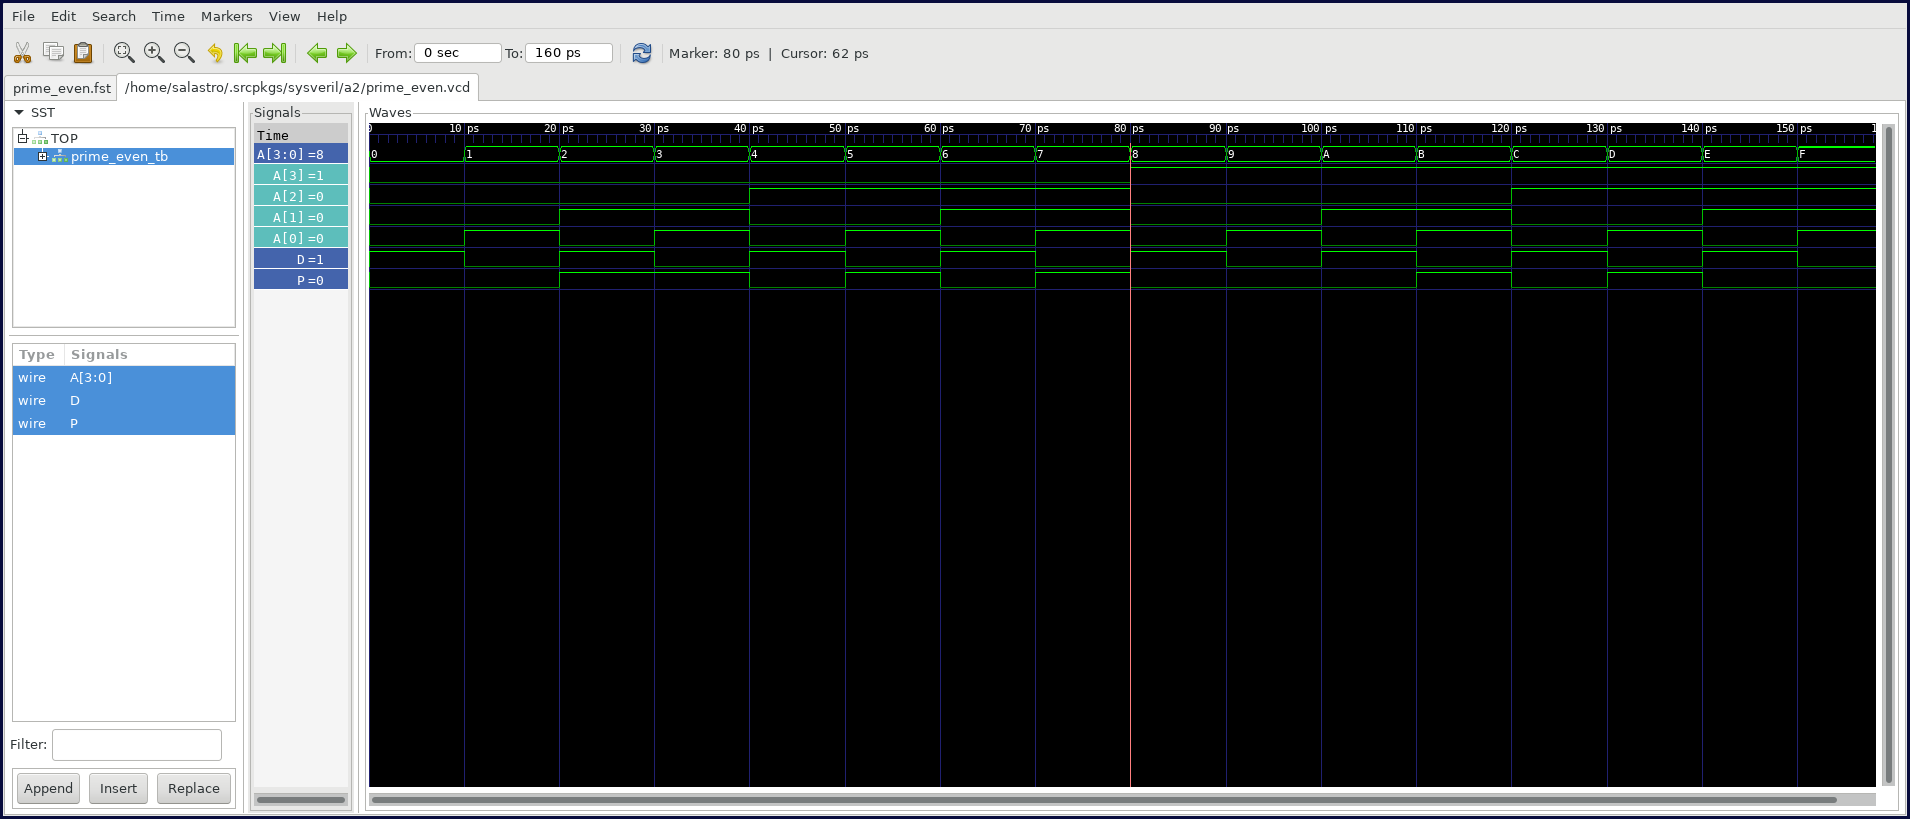
\includegraphics[width=0.7\textwidth]{waveform.png}
  \caption{Waveform of \texttt{prime\_even} using GTKWave}
  \label{fig:waveform-png}
\end{figure}

\begin{figure}[ht]
    \centering
    \incfig{\begin{figure}[ht]}
    \caption{\begin{figure}[ht]}
    \label{fig:\begin{figure}[ht]}
\end{figure}
    \centering
    \incfig{plot}
    \caption{plot}
    \label{fig:plot}
\end{figure}

\end{enumerate}

\end{document}
